\documentclass[11pt]{article}

\usepackage[letterpaper,margin=1in]{geometry}
\usepackage[T1]{fontenc}
\usepackage[utf8]{inputenc}
\usepackage{lmodern}
\usepackage{microtype}
\usepackage{amsmath,amssymb,amsthm,mathtools}
\usepackage{booktabs,longtable,array}
\usepackage{enumitem}
\usepackage{xcolor}
\usepackage{listings}
\usepackage{tikz}
\usetikzlibrary{arrows.meta,positioning,fit,calc}
\usepackage{fancyhdr}
\usepackage{url}
\newcommand{\doi}[1]{\href{https://doi.org/#1}{\nolinkurl{doi:#1}}}
\usepackage[colorlinks=true,linkcolor=blue!50!black,citecolor=green!35!black,urlcolor=blue!55!black]{hyperref}
\hypersetup{
  pdftitle={Contender 20: Autonomous W-Tree Universe Reflection},
  pdfauthor={Research proposal prepared for Vladimir Reshetnikov},
  pdfsubject={A kernel-checked large-number construction for BusyLean},
  pdfkeywords={Lean 4, large numbers, W-types, proof theory, reflection, BusyLean}
}
\usepackage[nameinlink,noabbrev]{cleveref}

\definecolor{codebg}{RGB}{247,248,250}
\definecolor{codeframe}{RGB}{210,214,220}
\definecolor{codekw}{RGB}{78,46,144}
\definecolor{codecomment}{RGB}{64,110,76}
\definecolor{codestring}{RGB}{150,65,55}
\definecolor{accent}{RGB}{31,78,121}

\lstdefinelanguage{Lean}{
  morekeywords={def,theorem,lemma,inductive,structure,instance,namespace,end,open,import,where,by,match,with,if,then,else,let,in,fun,forall,exists,abbrev,opaque,partial,termination_by,decreasing_by,deriving,do,return,have,show,exact,refine,intro,cases,case,simpa,simp,rw,apply,obtain,rcases,subst},
  sensitive=true,
  morecomment=[l]{--},
  morecomment=[s]{/-}{-/},
  morestring=[b]"
}

\lstset{
  language=Lean,
  basicstyle=\ttfamily\scriptsize,
  keywordstyle=\color{codekw}\bfseries,
  commentstyle=\color{codecomment},
  stringstyle=\color{codestring},
  backgroundcolor=\color{codebg},
  frame=single,
  rulecolor=\color{codeframe},
  breaklines=true,
  breakatwhitespace=false,
  columns=fullflexible,
  keepspaces=true,
  showstringspaces=false,
  tabsize=2,
  numbers=left,
  numberstyle=\tiny\color{gray},
  xleftmargin=1.8em,
  framexleftmargin=1.4em,
  aboveskip=0.8em,
  belowskip=0.8em,
  literate=
    {≤}{{$\leq$}}1
    {≥}{{$\geq$}}1
    {→}{{$\rightarrow$}}1
    {←}{{$\leftarrow$}}1
    {∀}{{$\forall$}}1
    {∃}{{$\exists$}}1
    {∈}{{$\in$}}1
    {∉}{{$\notin$}}1
    {∧}{{$\land$}}1
    {∨}{{$\lor$}}1
    {¬}{{$\neg$}}1
    {≠}{{$\neq$}}1
    {⟨}{{$\langle$}}1
    {⟩}{{$\rangle$}}1
    {Σ}{{$\Sigma$}}1
    {α}{{$\alpha$}}1
    {β}{{$\beta$}}1
    {ℕ}{{$\mathbb{N}$}}1
    {ω}{{$\omega$}}1
    {φ}{{$\varphi$}}1
    {Γ}{{$\Gamma$}}1
    {ε}{{$\varepsilon$}}1
    {≡}{{$\equiv$}}1
    {·}{{$\cdot$}}1
}

\newtheorem{theorem}{Theorem}[section]
\newtheorem{proposition}[theorem]{Proposition}
\newtheorem{lemma}[theorem]{Lemma}
\newtheorem{corollary}[theorem]{Corollary}
\theoremstyle{definition}
\newtheorem{definition}[theorem]{Definition}
\newtheorem{construction}[theorem]{Construction}
\theoremstyle{remark}
\newtheorem{remark}[theorem]{Remark}
\newtheorem{limitation}[theorem]{Limitation}

\newcommand{\BusyLean}{\textsc{BusyLean}}
\newcommand{\Lean}{\textsc{Lean}}
\newcommand{\WTree}{\mathsf{WTree}}
\newcommand{\Orb}{\operatorname{Orb}_{19}}
\newcommand{\reflectA}{\operatorname{Reflect}_{A}}
\newcommand{\diagLift}{\operatorname{DiagLift}}
\newcommand{\FinalCommit}{\texttt{fd43cae755356719c907fde0b0b131d258a30e18}}
\newcommand{\BaseCommit}{\texttt{64d31a0cf6f1aa4477a088be5554957de6e87a61}}
\newcommand{\DefinitionTime}{0.746 s}
\newcommand{\ProofTime}{0.454 s}
\newcommand{\PreviousTime}{20.061 s}
\newcommand{\WorkflowRun}{\texttt{38425930036}}

\pagestyle{fancy}
\fancyhf{}
\lhead{Autonomous W-tree universe reflection}
\rhead{Contender 20 proposal}
\cfoot{\thepage}
\setlength{\headheight}{14pt}

\title{\bfseries Contender 20: Autonomous W-Tree Universe Reflection\\[0.45em]
\large A kernel-checked large-number construction for \textnormal{\BusyLean}}
\author{Research proposal prepared for Vladimir Reshetnikov}
\date{13 October 2026}

\begin{document}
\maketitle

\begin{abstract}
We propose a new constructive natural number for the \BusyLean{} repository,
whose accepted baseline at the audited revision is Contender~19.  The new
construction replaces the explicit linearly ordered large-Veblen universe
ladder by a ramified hierarchy indexed by valid addresses in a
countably-branching well-founded W-tree generated from the repository's own
reflection machinery.  It then reflects a family of finite iterates of the
Contender~19 function through the repository's rank hierarchy of
hyperreflection lifts.  The resulting closed term is
\[
  N_{20} \;:=\; F_{20}\bigl(F_{20}(42)\bigr).
\]
All defining recursion is accepted by Lean 4.34.0 and is therefore total.  A
formal comparison proves
\[
  N_{19} < N_{20},
\]
and a stronger closed theorem proves that $N_{20}$ exceeds an $F_{19}$-orbit
whose length is itself $F_{20}(42)+2$:
\[
 F_{19}^{\,F_{20}(42)+2}\bigl(F_{20}(42)\bigr) < N_{20}.
\]
The definition, well-foundedness proof, strong-normalization instance,
comparison theorems, smoke tests, transitive dependency audit, and
contest-style timing script are included.  The successful audit uses only the
axioms \texttt{propext} and \texttt{Quot.sound}, the same permitted set used by
the repository.  We carefully separate these kernel-checked numerical claims
from the more speculative proof-theoretic interpretation of the new ramified
language.
\end{abstract}

\tableofcontents
\newpage

\section{Executive summary}

The proposal has two independent sources of growth.

\begin{enumerate}[leftmargin=2.2em]
\item \textbf{A new reflected language.}  The atom order of the existing
  predicative-universe language is instantiated with finite addresses in an
  autonomous W-tree.  Direct predecessors are valid immediate children.  The
  relation is non-linear and ramified, but structurally well-founded.  This
  yields a normalization theorem for a language whose universe levels follow
  the branching structure generated by \BusyLean's own W-tree machinery.

\item \textbf{A substantially stronger seed family.}  Instead of repeating
  Contender~19's family at every oracle coordinate, coordinate $i$ contains
  the $(i+2)$-fold iterate of $F_{19}$.  Rank and schedule are themselves fed
  by a very long member of that orbit.  A generic progressivity theorem then
  proves that $F_{20}(n)$ dominates every orbit coordinate visible through
  $n$.
\end{enumerate}

The exact Lean definition is
\begin{align*}
  \Orb(i,n) &:= F_{19}^{\,i+2}(n),\\
  h_{20}(n) &:= \Orb\bigl(F_{19}(F_{19}(n)),n\bigr),\\
  S_{20}(n) &:= \operatorname{realize}\!\left(
      \operatorname{hyper}_{h_{20}(n)+42}
      (\operatorname{encode}(T_{\!*}))\right),\\
  r_{20}(n) &:= h_{20}(n)+1,\\
  F_{20}(n) &:= \diagLift\bigl(S_{20}(n),r_{20}(n),
      \reflectA,\Orb,n,n\bigr),\\
  N_{20} &:= F_{20}(F_{20}(42)).
\end{align*}
Here $T_{\!*}$ is the autonomous universe tree defined in
\cref{sec:autonomous-tree}, and $\reflectA$ is finite reflection over the
corresponding object language.

\paragraph{Status.}
The final branch revision is \FinalCommit{}, based on main revision
\BaseCommit{}.  A clean contest-style validation run \WorkflowRun{} reports
incremental definition time \DefinitionTime{} and proof time \ProofTime{},
after prebuilding the accepted previous contender in \PreviousTime{}.

\section{Repository baseline and design target}
\label{sec:baseline}

At base revision \BaseCommit{}, the repository's README identifies
Contender~19 as the current entry.  Its language uses a predicative ladder
whose atoms are normal large-Veblen terms, and its amplifier is the generic
rank hierarchy of transformer lifts.  In schematic notation,
\[
  N_{19}=F_{19}(F_{19}(42)).
\]
The recent sequence of language extensions is summarized in
\cref{tab:baseline}.

\begin{table}[ht]
\centering
\caption{Recent \BusyLean{} universe ladders at the audited base revision.}
\label{tab:baseline}
\begin{tabular}{@{}lll@{}}
\toprule
Contender & Atom order / ladder length & Main certified comparison \\
\midrule
16 & Cantor-style atoms below $\omega^\omega$ & $N_{15}<N_{16}$ \\
17 & Cantor normal forms below $\varepsilon_0$ & $N_{16}<N_{17}$ \\
18 & hereditary Veblen terms below $\Gamma_0$ & $N_{17}<N_{18}$ \\
19 & Sch\"utte-style large-Veblen terms & $N_{18}<N_{19}$ \\
\bottomrule
\end{tabular}
\end{table}

The task is not satisfied by defining $N_{19}+1$ or by hiding the old number
inside an opaque wrapper.  We therefore impose five design requirements.

\begin{enumerate}[leftmargin=2.2em]
\item The new term must be a closed Lean natural number, with no external
  oracle and no non-terminating evaluator.
\item It must have an exact theorem of strict domination over Contender~19.
\item The strict comparison should not require an unproved monotonicity theorem
  for the very complicated reflection functions.
\item The construction should introduce a genuine new language-level idea,
  not only a larger numeral parameter.
\item The formal lower bound should demonstrate a gap much larger than one
  application of the previous function.
\end{enumerate}

The resulting design meets all five.  The numerical proof uses only generic
progressivity, while the language contribution is certified separately by a
theorem bounding every enumerated program.

\section{The ramified W-tree atom order}
\label{sec:wtree-order}

\subsection{Finite addresses}

Let $T:\WTree(\mathbb N)$ be a countably branching well-founded tree.  A finite
address is generated by
\[
  p ::= \epsilon \mid p\mathbin{\raisebox{0.15ex}{$\smallfrown$}}i,
  \qquad i\in\mathbb N.
\]
The Lean datatype \texttt{TreePath} uses \texttt{root} for $\epsilon$ and
\texttt{child p i} for appending branch $i$.  The partial operation
$\operatorname{follow}_T(p)$ traverses $T$ along $p$ and returns the reached
subtree when all requested branch steps exist.

\begin{definition}[Validity]
An address $p$ is \emph{valid in $T$} when
$\operatorname{follow}_T(p)$ returns a subtree.
\end{definition}

\begin{definition}[Immediate valid-child relation]
For addresses $a,b$, define $b\prec_T a$ precisely when
\[
  b=a\mathbin{\raisebox{0.15ex}{$\smallfrown$}}i
  \quad\text{for some }i,
  \qquad\text{and }b\text{ is valid in }T.
\]
This is the Boolean function \texttt{TreePath.childLt T b a}.
\end{definition}

The relation is deliberately the immediate-child relation, not its transitive
closure.  It is generally branching and non-linear.  A universe at address
$a$ directly sees its immediate valid children; deeper descendants are
available by repeated nesting through the child universes.  This is a
ramified accessibility graph rather than a conventional linear ordinal
notation system.

\subsection{Structural well-foundedness}

\begin{theorem}[Kernel theorem \texttt{childLt\_wf}]
For every $T:\WTree(\mathbb N)$, the relation $\prec_T$ is well-founded.
\end{theorem}

\begin{proof}[Proof architecture]
The stronger auxiliary theorem \texttt{acc\_follow} is proved by structural
recursion on a reached subtree $U$.

If $U$ is a leaf, no extension of the current address is valid, so the current
address has no predecessors.  If $U=\operatorname{node}(f)$, every predecessor
has the form $p\mathbin{\raisebox{0.15ex}{$\smallfrown$}}i$ and reaches $f(i)$;
its accessibility follows from the recursive call on that child subtree.
For an invalid address, the same contradiction shows that it has no valid
child predecessor.  Thus every address is accessible.
\end{proof}

This proof does not translate $T$ to an external ordinal, invoke choice, or
assume transitivity.  It follows the inductive structure already accepted by
Lean for \texttt{WTree}.

\subsection{Finite enumeration}

The evaluator must maximize over a finite list.  The function
\texttt{pathsUpTo} starts with the root and, at stage $n+1$, appends every
branch index below $n+1$ to every previously generated path.  Filtering by
validity gives \texttt{wLevelsUpTo n}.

Every finite address appears at some sufficiently large stage: choose a stage
larger than both the path length and every branch index occurring in it.  This
cofinality observation is elementary and is used only as an interpretation of
the enumeration; the numerical comparison theorems need merely the actual
finite lists produced at each input.

\section{The autonomous universe tree}
\label{sec:autonomous-tree}

The fixed tree used as the atom index is
\[
 T_{\!*}=\operatorname{node}(k\mapsto B_k),
\]
where
\begin{align*}
 B_0 &:= \texttt{tree12},\\
 B_{n+1} &:= \operatorname{realize}\!\left(
     \operatorname{hyper}_n(\operatorname{encode}(\texttt{tree12}))
   \right).
\end{align*}
The definitional theorem \texttt{follow\_tree12} verifies that branch zero is
exactly \texttt{tree12}.  In turn, \texttt{tree12} was built from the
language-generated index that joins W-trees denoted by the repository's
W-language programs.  Thus the new universe graph is not an unrelated fixed
ordinal notation imported from outside the project: it contains the existing
autonomous reflection tree and a countable family of finite hyper-closures
above it.

\begin{figure}[ht]
\centering
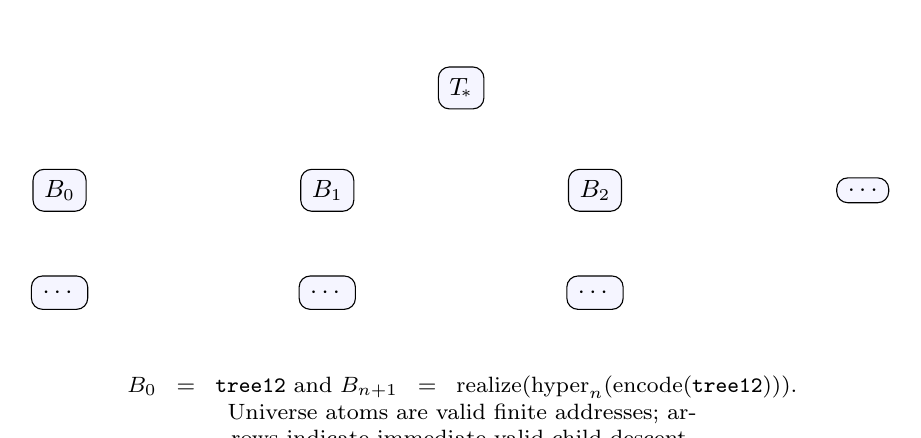
\begin{tikzpicture}[
  level distance=13mm,
  level 1/.style={sibling distance=34mm},
  level 2/.style={sibling distance=10mm},
  every node/.style={draw,rounded corners,fill=blue!4,inner sep=4pt,font=\small},
  edge from parent/.style={-Latex,thin},
  note/.style={draw=none,fill=none,font=\footnotesize,inner sep=1pt}
]
\node {$T_{\!*}$}
  child { node {$B_0$} child { node {$\cdots$} } }
  child { node {$B_1$} child { node {$\cdots$} } }
  child { node {$B_2$} child { node {$\cdots$} } }
  child { node {$\ldots$} };
\node[note,below=8mm of current bounding box.south,text width=0.9\linewidth,align=center]
  {$B_0=\texttt{tree12}$ and
   $B_{n+1}=\operatorname{realize}(\operatorname{hyper}_n(\operatorname{encode}(\texttt{tree12})))$.\\
   Universe atoms are valid finite addresses; arrows indicate immediate valid-child descent.};
\end{tikzpicture}
\caption{Schematic shape of the autonomous universe tree.  The diagram is
illustrative; every node is countably branching.}
\label{fig:tree}
\end{figure}

\begin{remark}[What is and is not proved]
The Lean development proves structural well-foundedness of the address
relation.  It does \emph{not} identify the order type of $T_{\!*}$ with a
standard named proof-theoretic ordinal, nor does it prove that this language
has greater proof-theoretic strength than the large-Veblen language.  Such a
calibration would be a separate research project.  Numerical domination of
Contender~19 is nevertheless exact and independent of that calibration.
\end{remark}

\section{A universe model over the W-tree levels}
\label{sec:language}

The repository's module \texttt{SystemFL/Transfinite.lean} is parametric in an
atom type equipped with a Boolean strict relation and a proof that the induced
relation is well-founded.  Its constructor \texttt{FL.wfUniv} builds a
predicative universe semantics by well-founded recursion, and
\texttt{FL.sn\_of\_typed} proves strong normalization of every typed term in
that universe.

We instantiate the generic atom interface by
\[
  \texttt{WLevel}:=\texttt{TreePath},
  \qquad
  \texttt{ALt}:=\prec_{T_{\!*}}.
\]
The theorem \texttt{wLevel\_wf} is immediate from \texttt{childLt\_wf}.  The
specialized strong-normalization theorem is:

\begin{theorem}[Kernel theorem \texttt{sn\_erase\_wlevel}]
If the checker infers natural-number type for a closed W-level term $t$, then
its erasure is strongly normalizing relative to every numerical oracle
$f:\mathbb N\to\mathbb N$.
\end{theorem}

The evaluator \texttt{FL.avalue} first type-checks a term with bounded fuel.  A
term inferred to have natural-number type is normalized using the certified
normalizer and decoded; every other case receives value zero.  At input $n$,
\texttt{autonomousLadderUpTo n} is a finite list of terms generated from the
finite atom list \texttt{wLevelsUpTo n} and syntax depth $n$.

\subsection{Why the non-linear order is semantically meaningful}

A linear ladder has one level below another.  Here a node may have many
incomparable children.  The generic universe construction handles this
without change: the semantic domain attached to a parent is formed from the
lower atoms named by the relation.  Since child domains are themselves
constructed recursively, a path of length $d$ gives $d$ layers of nested
universe access.  Siblings remain separate branches unless a higher parent
packages both.  This gives a genuine tree-shaped predicative hierarchy.

\section{Finite reflection over the autonomous language}
\label{sec:reflection}

For an oracle family $f:\mathbb N\to\mathbb N\to\mathbb N$, define
\begin{align*}
 M_{\mathrm{oracle}}(f,n)
   &:= \max_{0\leq i\leq n} f(i,n),\\
 M_{\mathrm{prog}}(f,n)
   &:= \max\{\operatorname{avalue}(\operatorname{packFamily}(f),n,t):
            t\in\operatorname{autonomousLadderUpTo}(n)\},\\
 \reflectA(f,n)
   &:= n+1+\max\bigl(M_{\mathrm{oracle}}(f,n),
                     M_{\mathrm{prog}}(f,n)\bigr).
\end{align*}
This is \texttt{reflectAFamily}; the corresponding transformer is
\texttt{aTransformer}.

\begin{proposition}[Exact one-step bounds]
For every $i\leq n$ and every enumerated term $t$ at depth $n$,
\begin{align*}
  f(i,n) &< \reflectA(f,n),\\
  \operatorname{avalue}(\operatorname{packFamily}(f),n,t)
    &< \reflectA(f,n).
\end{align*}
\end{proposition}

\begin{proof}
Both values lie below the corresponding finite maximum.  The additive guard
$n+1$ makes the result strictly larger.  The Lean theorems are
\nolinkurl{oracle_lt_reflectAFamily} and
\nolinkurl{avalue_lt_reflectAFamily}.
\end{proof}

Consequently \texttt{aTransformer} is \emph{progressive}: every visible
oracle coordinate is strictly increased.  This one property is precisely what
the generic hyperreflection comparison lemmas require.  No monotonicity of
$\reflectA$, $F_{19}$, or $F_{20}$ is assumed.

\section{The \texorpdfstring{$F_{19}$}{F19} orbit seed}
\label{sec:orbit}

Define finite iteration in the orientation
\[
  I_{19}(0,n)=n,
  \qquad
  I_{19}(k+1,n)=F_{19}(I_{19}(k,n)).
\]
Because the repository already proves $x<F_{19}(x)$ for every $x$, we obtain
\[
  I_{19}(k,n)<I_{19}(k+1,n)
\]
without any monotonicity theorem for $F_{19}$.

The family exposed to reflection is
\[
  \Orb(i,n):=I_{19}(i+2,n)=F_{19}^{\,i+2}(n).
\]
Coordinate zero is definitionally
\[
  \Orb(0,n)=F_{19}(F_{19}(n))=\texttt{family19}(n),
\]
so at $n=42$ it is exactly Contender~19.  Higher coordinates are strictly
larger finite iterates.

The schedule and rank are self-fed using
\[
  h_{20}(n):=\Orb(\texttt{family19}(n),n).
\]
Thus even before hyperreflection begins, the rank parameter is based on an
$F_{19}$ orbit whose iteration count is itself the previous contender family.
We then set
\begin{align*}
 S_{20}(n)&:=\operatorname{realize}\left(
     \operatorname{hyper}_{h_{20}(n)+42}
       (\operatorname{encode}(T_{\!*}))\right),\\
 r_{20}(n)&:=h_{20}(n)+1.
\end{align*}

\section{Definition of Contender 20}
\label{sec:def20}

The generic rank hierarchy \texttt{diagonalLift} repeatedly lifts a progressive
transformer along a W-tree schedule and across a natural-number rank.  We
instantiate it by the autonomous-language reflector and the $F_{19}$ orbit:
\[
  F_{20}(n):=
  \diagLift\bigl(S_{20}(n),r_{20}(n),\reflectA,\Orb,n,n\bigr).
\]
The proposed number is
\[
  \boxed{N_{20}:=F_{20}(F_{20}(42)).}
\]
The corresponding Lean fragment is short because the heavy lifting is in the
reusable language semantics, W-tree infrastructure, and generic
hyperreflection theorems.

\begin{lstlisting}[caption={Core definition of Contender 20.},label={lst:core}]
def orbit19 : Family := fun i n => iterateF19 (i + 2) n

def seedHeight20 (n : Nat) : Nat := orbit19 (family19 n) n

def schedule20 (n : Nat) : WTree Nat :=
  Autonomous.realize
    (Autonomous.hyper (seedHeight20 n + 42)
      (Autonomous.encode Ordinal.autonomousUniverseTree))

def rank20 (n : Nat) : Nat := seedHeight20 n + 1

def F20 (n : Nat) : Nat :=
  diagonalLift (schedule20 n) (rank20 n)
    aTransformer orbit19 n n

def contender_20 : Nat := F20 (F20 42)
\end{lstlisting}

\section{Exact comparison theorems}
\label{sec:comparison}

\subsection{Pointwise orbit domination}

The generic theorem \texttt{diagonalLift\_preservesProgressive} says that a
ranked lift of a progressive transformer still exceeds every visible oracle
coordinate.  Instantiating it yields the central pointwise estimate.

\begin{theorem}[Kernel theorem \texttt{orbit19\_lt\_F20}]
For all $i,n\in\mathbb N$,
\[
  i\leq n \quad\Longrightarrow\quad \Orb(i,n)<F_{20}(n).
\]
\end{theorem}

This immediately gives several concrete consequences.

\begin{corollary}[Previous-family domination]
For every $n$,
\[
  F_{19}(F_{19}(n))<F_{20}(n).
\]
\end{corollary}

\begin{corollary}[A visible 44-fold orbit at the contest input]
\[
  F_{19}^{44}(42)<F_{20}(42).
\]
\end{corollary}

\begin{corollary}[Program domination]
Every autonomous-ladder program enumerated at depth at most $n$, evaluated
with the packed orbit oracle, has value below $F_{20}(n)$.
\end{corollary}

The last statement is the theorem \texttt{avalue\_lt\_F20}; it isolates the
contribution of the new language from the seed comparison.

\subsection{Strict domination of Contender 19}

The repository's existing theorem $x<F_{19}(x)$ gives
\[
  n<F_{19}(n)<F_{19}(F_{19}(n))<F_{20}(n).
\]
Hence $F_{20}$ is strictly inflationary even though no general monotonicity
property is needed.  At $n=42$,
\[
  N_{19}=F_{19}(F_{19}(42))<F_{20}(42).
\]
Applying inflationarity at the argument $F_{20}(42)$ gives
\[
  F_{20}(42)<F_{20}(F_{20}(42))=N_{20}.
\]
Transitivity proves the required theorem.

\begin{theorem}[Kernel theorem
\texttt{contender\_19\_lt\_contender\_20}]
\[
  N_{19}<N_{20}.
\]
\end{theorem}

Since the repository has already chained each preceding contender into
Contender~19, transitivity places every accepted earlier contender below the
new number.

\subsection{A much stronger closed lower bound}

Use the pointwise orbit theorem at
\[
  n=i=F_{20}(42).
\]
Then
\[
 \Orb(F_{20}(42),F_{20}(42))
 =F_{19}^{\,F_{20}(42)+2}(F_{20}(42))
 <F_{20}(F_{20}(42))=N_{20}.
\]

\begin{theorem}[Kernel theorem
\texttt{long\_F19\_orbit\_lt\_contender\_20}]
\[
  F_{19}^{\,F_{20}(42)+2}(F_{20}(42))<N_{20}.
\]
\end{theorem}

This theorem is the principal formal answer to the word ``significantly.''
The gap is not a successor, a fixed finite iterate, or a single application of
the previous construction.  The number of $F_{19}$ iterations in the lower
bound is itself the already enormous value $F_{20}(42)+2$.

\section{Computability in principle}
\label{sec:computability}

The construction is not intended for practical evaluation.  Nevertheless it
is a computable natural number in the ordinary constructive sense represented
by Lean definitions.

\begin{proposition}
\texttt{contender\_20} denotes a total, closed value of type \texttt{Nat}.
\end{proposition}

\begin{proof}[Computational audit]
Each component is computationally finite at each natural input.

\begin{enumerate}[leftmargin=2.2em]
\item \texttt{TreePath.follow}, \texttt{pathsUpTo}, \texttt{iterateF19}, and
  all natural rank iterations are structurally recursive.
\item \texttt{wLevelsUpTo n}, \texttt{autonomousLadderUpTo n}, and every
  maximum used by reflection are finite lists computed from $n$.
\item The object-language evaluator runs only after a finite type-check.  Its
  normalizer is obtained from a constructive strong-normalization proof for
  the well-founded W-level universe.
\item W-trees are inductive values with functional branches.  A finite address
  or a structurally recursive fold inspects only the finitely demanded part of
  a branch function.
\item Lean's termination checker accepts every recursive definition in the
  transitive closure of \texttt{contender\_20}; there is no \texttt{partial},
  unsafe nontermination, unbounded search, or external oracle in the new
  modules.
\end{enumerate}

Therefore evaluation terminates in principle.  The required resources are far
beyond physical feasibility, which is the intended situation for a large
number contest.
\end{proof}

\begin{remark}
A proof of totality does not imply that the kernel should reduce the contest
input.  The development intentionally proves inequalities symbolically and
contains no \texttt{\#eval contender\_20} command.
\end{remark}

\section{Axiom, dependency, and build audit}
\label{sec:audit}

The focused audit prints the axioms of the main number, the exact comparison,
the orbit bounds, the language-value bound, the W-level well-foundedness proof,
and the specialized strong-normalization theorem.  At final revision
\FinalCommit{}, the permitted axioms are exactly
\[
  \{\texttt{propext},\texttt{Quot.sound}\}.
\]
The W-level well-foundedness theorem itself uses only \texttt{propext}.  No
choice principle, excluded-middle axiom constant, or user-declared axiom is
reported.

The transitive closure checker also verifies that the definition of
\texttt{contender\_20} does not mention any named constant
\texttt{contender\_5} through \texttt{contender\_19}.  This is not a claim that
it is independent of the preceding machinery: it intentionally uses the
function $F_{19}$ and reusable modules.  Rather, it follows the repository's
convention of rebuilding the previous family from its functional definition
instead of embedding the old closed contender constant.

\begin{table}[ht]
\centering
\caption{Contest-style validation phases on the GitHub Actions runner.  The
previous contender is prebuilt and is not charged to the new entry.}
\label{tab:timing}
\begin{tabular}{@{}lrrl@{}}
\toprule
Phase & Observed & Budget & Result \\
\midrule
Prebuild through \texttt{Comparison19} & \PreviousTime{} & not charged & pass \\
New definitions through \texttt{Contender20} & \DefinitionTime{} & 15 s & pass \\
New proofs through \texttt{Comparison20} & \ProofTime{} & 60 s & pass \\
Smoke and axiom/dependency audit & -- & -- & pass \\
\bottomrule
\end{tabular}
\end{table}

Exact wall-clock times depend on runner load and are engineering measurements,
not mathematical claims.  The reproducible script
\texttt{scripts/check\_contender20.py} deletes generated build directories,
prebuilds the accepted predecessor, times the two incremental phases, then
runs the smoke and audit files.

\section{Proof-theoretic interpretation}
\label{sec:interpretation}

W-types are a natural representation of well-founded branching constructions
in type theory and constructive set-theoretic interpretations
\cite{Aczel1978,Aczel1986}.  Ordinal analysis commonly uses well-founded
notation systems to organize iterated reflection, normalization, and
provably recursive growth; Sch\"utte's autonomous systems and Veblen methods
are classical examples \cite{Schuette1977}, while Buchholz-style collapsing
functions and later surveys extend the methodology far beyond predicative
analysis \cite{Buchholz1986,Rathjen2007,Rathjen1999}.

The present construction belongs to that tradition only in a broad structural
sense.  It combines:

\begin{itemize}[leftmargin=2.2em]
\item an internally generated well-founded branching index;
\item a universe semantics defined by recursion over that index;
\item finite reflection over programs normalized in the resulting language;
\item higher-order iteration of the reflector along W-tree schedules.
\end{itemize}

However, no standard ordinal assignment for the complete construction is
proved.  In particular, it would be unjustified to advertise $T_{\!*}$ as
``the Bachmann--Howard ordinal,'' ``beyond the large Veblen ordinal,'' or any
other named benchmark solely from its syntax.  The exact scientific result is
the Lean-certified numerical comparison and program bound.  The ordinal
calibration remains an open problem.

\section{Why this is not a toy successor trick}

Three features distinguish the proposal from a vacuous enlargement.

\paragraph{Language change.}
The object language no longer has a linearly ordered explicit atom notation.
It is interpreted over a branching universe graph containing the project's
autonomous W-tree index.  The well-foundedness and normalization instances are
new formal content.

\paragraph{Orbit seed.}
The oracle coordinates expose unboundedly many finite iterates of $F_{19}$.
At input $n$, the new reflection beats all coordinates through $n$, and the
rank and schedule are fed by an orbit coordinate indexed by the previous
family itself.

\paragraph{Closed strong lower bound.}
The theorem
\[
  F_{19}^{\,F_{20}(42)+2}(F_{20}(42))<N_{20}
\]
is internal to Lean.  It exhibits a gap that cannot be reduced to adding one
or applying $F_{19}$ a fixed number of extra times.

At the same time, the comparison proof remains robust: it depends on
progressivity and strict inflationarity, not on a delicate global monotonicity
theorem for the reflection hierarchy.

\section{Limitations and scope}
\label{sec:limitations}

\begin{limitation}[No exact ordinal calibration]
The formal development proves well-foundedness, not a named order type or a
proof-theoretic ordinal for the language.  Claims about relative language
strength beyond the stated Lean inequalities are heuristic.
\end{limitation}

\begin{limitation}[Immediate-child order]
The atom relation is not the transitive ancestor order.  Each universe directly
sees immediate children, with deeper access obtained through nesting.  A
transitive-closure variant may be stronger or easier to calibrate, but it would
require additional enumeration and comparison work.
\end{limitation}

\begin{limitation}[Language and seed are not separated by a dominance theorem]
The exact theorem $N_{19}<N_{20}$ is obtained from the orbit seed plus generic
progressivity.  The theorem \texttt{avalue\_lt\_F20} certifies that the new
language is reflected, but there is not yet a formal embedding theorem showing
that it strictly contains the large-Veblen language.
\end{limitation}

\begin{limitation}[No practical evaluation]
Only tiny smoke examples are evaluated.  The contest value is beyond feasible
execution, and the article gives no decimal expansion, residue, or runtime
estimate for it.
\end{limitation}

\begin{limitation}[Enumeration is intentionally redundant]
\texttt{pathsUpTo} may generate duplicate paths before filtering.  Duplicates
do not affect maxima or correctness, but a canonical breadth/size enumeration
would reduce small-input overhead.
\end{limitation}

\section{Further research questions}
\label{sec:future}

\begin{enumerate}[leftmargin=2.2em]
\item \textbf{Transitive W-tree ladders.}  Replace immediate-child order by the
  nonempty transitive closure of valid descent, prove well-foundedness in Lean,
  and compare the resulting universe semantics.

\item \textbf{Embedding large-Veblen atoms.}  Construct a certified
  order-preserving map from \nolinkurl{Ordinal.LargeVeblen} into valid addresses
  of a suitable autonomous tree.  This would separate a genuine language
  extension theorem from seed-based numerical domination.

\item \textbf{Ordinal calibration.}  Assign standard ordinal diagrams or
  collapsing-function terms to autonomous W-tree schedules, with soundness and
  cofinality theorems.  Determine which parts of the current hierarchy admit a
  recognizable proof-theoretic benchmark.

\item \textbf{Tree-indexed generic reflection theorem.}  Package the present
  construction as a reusable functor taking any enumerated well-founded W-tree
  to a normalized ladder language, reflector, and program bound.

\item \textbf{Self-hosted atom generation.}  Let the object language define or
  select its own level tree under a guarded universe discipline, rather than
  using a fixed external \texttt{autonomousUniverseTree}.

\item \textbf{Stronger orbit families.}  Replace finite $F_{19}$ iteration by
  a certified two-parameter diagonal hierarchy built from $F_{19}$, while
  retaining a simple comparison theorem that avoids monotonicity assumptions.

\item \textbf{Small-input profiling.}  Deduplicate path enumeration, memoize
  type generation, and measure the largest feasible tiny cases without ever
  attempting the contest input.

\item \textbf{Formal audit infrastructure.}  Move the transitive constant
  closure checker and permitted-axiom policy into a reusable repository module
  so each contender obtains the same machine-checked submission certificate.

\item \textbf{Independent proof review.}  Mechanically minimize imports and
  restate the key domination theorem in a small standalone file, reducing the
  trusted review surface.
\end{enumerate}

\section{Integration and reproduction}
\label{sec:reproduce}

The archive mirrors repository-relative paths.  From a checkout of BusyLean at
base revision \BaseCommit{}, copy the supplied files into place and run:

\begin{lstlisting}[language={},numbers=none]
python3 scripts/check_contender20.py
\end{lstlisting}

The script performs the following sequence.

\begin{enumerate}[leftmargin=2.2em]
\item Delete the main and embedded proposal build directories.
\item Build \texttt{BusyLean.Comparison19} as the accepted predecessor.
\item Time \texttt{BusyLean.Contender20} against the 15-second definition
  budget.
\item Time \texttt{BusyLean.Comparison20} against the 60-second proof budget.
\item Run \texttt{test/WTreeLadderSmoke.lean}.
\item Run \texttt{test/Contender20Audit.lean} and reject unpermitted axioms.
\end{enumerate}

For full repository integration, add imports for \texttt{Contender20} and
\texttt{Comparison20} to the relevant umbrella modules, extend the main audit
with the new declarations, and update the top-level README only after review.
The research branch is intentionally isolated; no merge into \texttt{main} is
part of this artifact.

\section{Conclusion}

Contender~20 combines a new ramified, internally generated universe index with
a self-fed orbit of the strongest existing BusyLean function.  Its key
mathematical infrastructure---W-tree address well-foundedness, specialization
of the generic universe model, finite program reflection, and orbit
progressivity---is formalized in Lean.  The exact comparison
$N_{19}<N_{20}$ is strengthened to a closed lower bound by an $F_{19}$ orbit of
length $F_{20}(42)+2$.  Every component is total and finite at each input, so
the number is computable in principle, while its evaluation is deliberately
out of practical reach.

The proposal therefore advances both dimensions relevant to a serious
large-number entry: it introduces a reusable formal mechanism rather than a
cosmetic wrapper, and it provides a transparent kernel-checked certificate of
a very large quantitative gap.

\appendix

\section{Lean source: W-tree atom order}
\label{app:wtree}
\lstinputlisting[caption={\texttt{BusyLean/Ordinal/WTreeLadder.lean}}]{../BusyLean/Ordinal/WTreeLadder.lean}

\section{Lean source: definition}
\label{app:def}
\lstinputlisting[caption={\texttt{BusyLean/Contender20.lean}}]{../BusyLean/Contender20.lean}

\section{Lean source: comparison theorems}
\label{app:comparison}
\lstinputlisting[caption={\texttt{BusyLean/Comparison20.lean}}]{../BusyLean/Comparison20.lean}

\section{Validation entry points}
\label{app:validation}
The archive also contains the complete smoke test, focused axiom/dependency
audit, contest-style timing script, GitHub Actions workflow, integration patch,
and recorded validation log.  Keeping these as executable artifacts rather
than reprinting them here avoids duplicating operational code in the article.

\begin{thebibliography}{Rathjen 2007}

\bibitem[Aczel 1978]{Aczel1978}
Peter Aczel.
\newblock The type theoretic interpretation of constructive set theory.
\newblock In Angus Macintyre, Leszek Pacholski, and Jeff Paris, editors,
  \emph{Logic Colloquium '77}, volume 96 of \emph{Studies in Logic and the
  Foundations of Mathematics}, pages 55--66. North-Holland, 1978.
\newblock \doi{10.1016/S0049-237X(08)71989-X}.

\bibitem[Aczel 1986]{Aczel1986}
Peter Aczel.
\newblock The type theoretic interpretation of constructive set theory:
  Inductive definitions.
\newblock In \emph{Logic, Methodology and Philosophy of Science VII}, volume
  114 of \emph{Studies in Logic and the Foundations of Mathematics}, pages
  17--49. Elsevier, 1986.
\newblock \doi{10.1016/S0049-237X(09)70683-4}.

\bibitem[Buchholz 1986]{Buchholz1986}
Wilfried Buchholz.
\newblock A new system of proof-theoretic ordinal functions.
\newblock \emph{Annals of Pure and Applied Logic}, 32:195--207, 1986.
\newblock \doi{10.1016/0168-0072(86)90052-7}.

\bibitem[Rathjen 1999]{Rathjen1999}
Michael Rathjen.
\newblock The realm of ordinal analysis.
\newblock In S. Barry Cooper and John K. Truss, editors, \emph{Sets and
  Proofs}, pages 219--280. Cambridge University Press, 1999.
\newblock \doi{10.1017/CBO9781107325944.011}.

\bibitem[Rathjen 2007]{Rathjen2007}
Michael Rathjen.
\newblock The art of ordinal analysis.
\newblock In \emph{Proceedings of the International Congress of
  Mathematicians, Madrid 2006, Volume II}, pages 45--69. European Mathematical
  Society, 2007.
\newblock \doi{10.4171/022-2/3}.

\bibitem[Sch\"utte 1977]{Schuette1977}
Kurt Sch\"utte.
\newblock \emph{Proof Theory}.
\newblock Grundlehren der mathematischen Wissenschaften 225. Springer-Verlag,
  Berlin, Heidelberg, and New York, 1977.
\newblock \doi{10.1007/978-3-642-66473-1}.

\end{thebibliography}

\end{document}
